\documentclass{article}
\usepackage{amsmath}
\usepackage{amsfonts}
\usepackage{amssymb}
\usepackage{amsmath}
\usepackage{mathrsfs}
\usepackage{bm}
\usepackage{changepage}
\usepackage{framed}
\usepackage{geometry}
\usepackage{inputenc}
\usepackage{amsthm}
\usepackage{mathtools}
\usepackage{esint}
\usepackage{marvosym}
\usepackage{xcolor}

\title{Math 4500 HW \#01 Solutions}
\author{Instructor: Birgit Speh\\ TA: Guanyu Li}
\date{}
\geometry{left=2cm,right=2cm,top=2.5cm,bottom=2.5cm}

\theoremstyle{definition}
\newtheorem{problem}{Problem}
\theoremstyle{plain}
\newtheorem*{remark}{Remark}

\begin{document}

\maketitle\par

\emph{This solution set is not error-free. Please email me (gl479\MVAt cornell.edu) if you spot any errors or typos!}

\begin{problem}[Exercise 1.2.4 (5 pts)]Deduce, from the distributive law and multiplicative absolute value, that
\begin{displaymath}
|uv-uw|=|u||v-w|.
\end{displaymath}
Explain why this says that multiplication of the whole plane of complex numbers by $u$ multiplies all distances by $|u|$.
\end{problem}
\begin{adjustwidth}{0.7cm}{}
\color{blue}
\begin{proof}[Solution]
\begin{align*}
|uv-uw|=|u(v-w)|=|u||v-w|.^{[2]}
\end{align*}
Suppose $v,w$ are two points in the complex plane, then $|v-w|$ represents the distance between two points and $|uv-uw|$ represents the distance between points after the transformation that multiplying the whole plane by $u.^{[2]}$ The equation means that the distance changes with a parameter $|u|.^{[1]}$
\end{proof}
\color{black}
\end{adjustwidth}
~\par

\begin{problem}[Exercise 1.2.5 (5 pts)]Deduce from Exercise 1.2.4 that multiplication of the whole plane of complex numbers by $\cos\theta+i\sin\theta$ leaves all distances unchanged.
\end{problem}
\begin{adjustwidth}{0.7cm}{}
\color{blue}
\begin{proof}[Solution]Denote $u=\cos\theta+i\sin\theta$ then $|u|=\cos^2\theta+\sin^2\theta=1.^{[2]}$ Suppose $v,w$ are two points in the complex plane, then by previous exercise $|uv-uw|=|u||v-w|=|v-w|,^{[1]}$ where $|v-w|$ represents the distance between previous points and $|uv-uw|$ means the distance between the new points. Hence the transformation leaves all distances unchanged$.^{[2]}$
\end{proof}
\color{black}
\end{adjustwidth}
~\par

\begin{problem}[Exercise 1.3.6 (10 pts)]Show that the multiplicative property of determinants gives the \emph{real four-square identity}
\begin{align*}
(a_1^2+b_1^2+c_1^2+d_1^2)(a_2^2+b_2^2+c_2^2+d_2^2)&=(a_1a_2-b_1b_2-c_1c_2-d_1d_2)^2+(a_1b_2+b_1a_2+c_1d_2-d_1c_2)^2\\
&\phantom{=}+(a_1c_2-b_1d_2+c_1a_2+d_1b_2)^2+(a_1d_2+b_1c_2-c_1b_2+d_1a_2)^2
\end{align*}
\end{problem}
\begin{adjustwidth}{0.7cm}{}
\color{blue}
\begin{proof}[Solution]Let $\alpha:=\begin{pmatrix}a_1+id_1&-b_1-ic_1\\ b_1-ic_1&a_1-id_1\end{pmatrix}$ and $\beta:=\begin{pmatrix}a_2+id_2&-b_2-ic_2\\ b_2-ic_2&a_2-id_2\end{pmatrix}$. Then the determinants gives
\begin{displaymath}
|\alpha||\beta|=|\alpha\beta|,^{[3]}
\end{displaymath}
where the left hand side is just
\begin{displaymath}
(a_1^2+b_1^2+c_1^2+d_1^2)(a_2^2+b_2^2+c_2^2+d_2^2).^{[2]}
\end{displaymath}
On the other hand, the right hand side is
\begin{align*}
|\alpha\beta|&=\det\left(\begin{pmatrix}a_1+id_1&-b_1-ic_1\\ b_1-ic_1&a_1-id_1\end{pmatrix}\begin{pmatrix}a_2+id_2&-b_2-ic_2\\ b_2-ic_2&a_2-id_2\end{pmatrix}\right)\\
&=\det\begin{pmatrix}(a_1+id_1)(a_2+id_2)+(-b_1-ic_1)(b_2-ic_2)&(a_1+id_1)(-b_2-ic_2)+(-b_1-ic_1)(a_2-id_2)\\ (a_1+id_1)(b_1-ic_1)+(a_1-id_1)(b_2-ic_2)&(-b_2-ic_2)(b_1-ic_1)+(a_1-id_1)(a_2-id_2)\end{pmatrix}\\
&=\det\begin{pmatrix}(a_1a_2-a_1d_2-b_1b_2-c_1c_2)+i(a_2d_1+a_1d_2+c_2b_1-c_1b_2)&-(a_1b_2+b_1a_2+c_1d_2-d_1c_2)-i(a_1c_2-b_1d_2+c_1a_2+d_1b_2)\\ -(a_1b_2+b_1a_2+c_1d_2-d_1c_2)+i(a_1c_2-b_1d_2+c_1a_2+d_1b_2)&(a_1a_2-a_1d_2-b_1b_2-c_1c_2)+i(a_2d_1+a_1d_2+c_2b_1-c_1b_2)\end{pmatrix}\\
=RHS.^{[5]}
\end{align*}
\end{proof}
\color{black}
\end{adjustwidth}

\begin{problem}[Exercise 1.4.4 (10 pts)]
Also deduce the \emph{Jacobi identity} for the cross product:
\begin{displaymath}
u\times(v\times w)+w\times(u\times v)+v\times(w\times u)=0.
\end{displaymath}
The antisymmetric and Jacobi properties show that the cross product is not completely lawless. These properties define what we later call a \emph{Lie algebra}.
\end{problem}
\begin{adjustwidth}{0.7cm}{}
\color{blue}
\begin{proof}[Solution]We first verify the identity
\begin{displaymath}
u\times(v\times w)=(w\cdot u)v-(u\cdot v)w.
\end{displaymath}
Suppose that $u=u_1\bm{\mathrm{i}}+u_2\bm{\mathrm{j}}+u_3\bm{\mathrm{k}}$, $v=v_1\bm{\mathrm{i}}+v_2\bm{\mathrm{j}}+v_3\bm{\mathrm{k}}$ and $w=w_1\bm{\mathrm{i}}+w_2\bm{\mathrm{j}}+w_3\bm{\mathrm{k}}$. By definition, we have
\begin{align*}
u\times(v\times w)&=u\times((v_2w_3-v_3w_2)\bm{\mathrm{i}}+(v_3w_1-v_1w_3)\bm{\mathrm{j}}+(v_1w_2-v_2w_1)\bm{\mathrm{k}})\\
&=(u_2(v_1w_2-v_2w_1)-u_3(v_3w_1-v_1w_3))\bm{\mathrm{i}}\\
&\phantom{=}+(u_3(v_2w_3-v_3w_2)-u_1(v_1w_2-v_2w_1))\bm{\mathrm{j}}\\
&\phantom{=}+(u_1(v_3w_1-v_1w_3)-u_2(v_2w_3-v_3w_2))\bm{\mathrm{k}}\\
&=((u_2w_2+u_3w_3)v_1-(u_2v_2+u_3v_3)w_1)\bm{\mathrm{i}}\\
&\phantom{=}+((u_3w_3+u_1w_1)v_2-(u_3v_3+u_1v_1)w_2)\bm{\mathrm{j}}\\
&\phantom{=}+((u_1w_1+u_2w_2)v_3-(u_1v_1+u_2v_2)w_3)\bm{\mathrm{k}}\\
&=((u_1w_1+u_2w_2+u_3w_3)v_1-(u_1v_1+u_2v_2+u_3v_3)w_1)\bm{\mathrm{i}}\\
&\phantom{=}+((u_2w_2+u_3w_3+u_1w_1)v_2-(u_2v_2+u_3v_3+u_1v_1)w_2)\bm{\mathrm{j}}\\
&\phantom{=}+((u_3w_3+u_1w_1+u_2w_2)v_3-(u_3v_3+u_1v_1+u_2v_2)w_3)\bm{\mathrm{k}}\\
&=(w\cdot u)v-(u\cdot v)w.^{[7]}
\end{align*}\par
Back to the problem,
\begin{align*}
&\phantom{=}u\times(v\times w)+w\times(u\times v)+v\times(w\times u)\\
&=((w\cdot u)v-(u\cdot v)w)+((v\cdot w)u-(w\cdot u)v)+((u\cdot v)w-(v\cdot w)u)\\
&=0.^{[3]}
\end{align*}
\end{proof}
\color{black}
\end{adjustwidth}
~\par

\begin{remark}If your find Exercise 1.5.5 and 1.5.6 hard to guess/prove the answer, go to do Exercise 1.5.1-1.5.4. The 2-dimensional case would tell you everything.
\end{remark}

\begin{problem}[Exercise 1.5.5 (20 pts)]Adapt the argument of Exercise 1.5.3 to great circles $\mathscr{L},\mathscr{M},\mathscr{N}$ shown in the picture. What is the conclusion?
\begin{figure}[h]
\centering
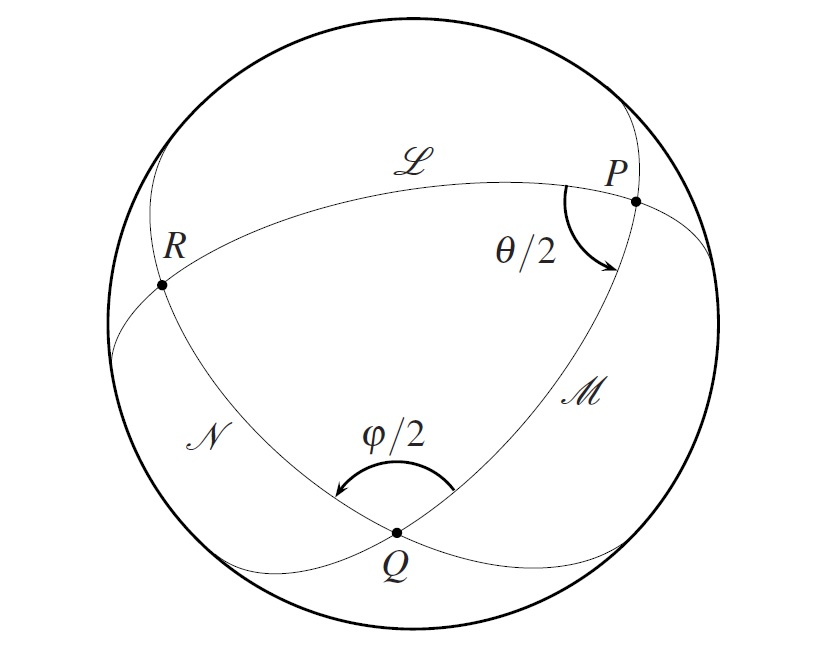
\includegraphics[scale=0.7]{hw1p.jpg}
\caption{Reflection in great circles on the sphere}
\end{figure}
\end{problem}
\begin{adjustwidth}{0.7cm}{}
\color{blue}
\begin{proof}[Solution]Literally there are two conclusions: (i) any rotation can be decomposed as a composition of two reflections, and the composition of two reflections is a rotation; (ii) two rotations make a rotation (or all rotations form a group with the multiplication being the composition of maps)$.^{[5]}$\\~\par
Suppose $A$ is a rotation about a line $l$ through the origin. Let $l\cap S^2=\{P,Q\}$, and let $\mathscr{M}$ be an ARBITRARY great circle through $P$ and $Q$. Also we use $\mathscr{M}$ to denote the plane through the line $l$. Let $\mathscr{L}$ be another great circle through $P$ and $Q$ s.t. the angle between $\mathscr{M}$ and $\mathscr{N}$ is $\theta/2$ where $\theta$ is the rotation angle. Let $x$ be an arbitrary point, and let $x'$ be the point of $x$ reflected by the great circle $\mathscr{L}$, and let $x''$ be the point of $x'$ reflected by the great circle $\mathscr{M}$. Then $\angle xPx''=2\frac{\theta}{2}=\theta$, and $|xP|=|x''P|$. Hence $A$ can be decomposed as the composition of reflections, by the great circle $\mathscr{M}$ and by the great circle $\mathscr{M}$ respectively. The same argument proves that the composition of two reflections is a rotation$.^{[10]}$\par
Suppose $A_1,A_2$ are two given rotations, and $P,Q$ are points fixed by $A_1,A_2$ respectively. As shown in the picture, denote the great circle through points $P,Q$ as $\mathscr{M}$. Let $\mathscr{L},\mathscr{N}$ are the great circles s.t. the angle from $\mathscr{L}$ to $\mathscr{M}$ is $\frac{\theta}{2}$ and the angle from $\mathscr{M}$ to $\mathscr{N}$ is $\frac{\varphi}{2}$, where $\theta,\varphi$ are the angle of the rotations. By abuse of notation, we also denote the reflection by great circles $\mathscr{L},\mathscr{M},\mathscr{N}$ as $\mathscr{L},\mathscr{M},\mathscr{N}$. Hence by the first conclusion,
\begin{displaymath}
A_1=\mathscr{M}\circ\mathscr{L},~A_2=\mathscr{N}\circ\mathscr{M}.
\end{displaymath}
Therefore
\begin{displaymath}
A_2\circ A_1=\mathscr{N}\circ\mathscr{M}\circ\mathscr{M}\circ\mathscr{L}=\mathscr{N}\circ\mathscr{L},
\end{displaymath}
which implies $A_2\circ A_1$ is again a rotation$.^{[5]}$
\end{proof}
\color{black}
\end{adjustwidth}
~\par

\begin{problem}[Exercise 1.5.6 (5 pts)]Explain why there is no exceptional case analogous to Exercise 1.5.4. Deduce that the product of any two rotations of $\mathbb{R}^3$ about $O$ is another rotation, and explain how to find the axis of the product rotation.
\end{problem}
\begin{adjustwidth}{0.7cm}{}
\color{blue}
\begin{proof}[Solution]Suppose we have three planes $\mathscr{L},\mathscr{M},\mathscr{N}$ in the space going through the origin, then any two of them (w.l.o.g. assume they are $\mathscr{L}$ and $\mathscr{M}$) intersect, so their intersection is a line denoted by $l$. Suppose $l$ intersects the unit sphere at a point $R$, then $R$ is an intersection point of the great circles which are the intersections $\mathscr{L}\cap S^2$ and $\mathscr{M}\cap S^2$, where $S^2$ denotes the sphere$.^{[5]}$
\end{proof}
\color{black}
\end{adjustwidth}

\begin{remark}Generally it is not OK to use some statement that you cannot prove. It is a truth that on a sphere there cannot be parallel geodesics. But it requires a lot to define what is a geodesic and to actually prove the proposition. So if you want to use some fancy things in the homework, explicitly write down everything, every definition and every proof.
\end{remark}
~\par

\begin{problem}[Exercise 2.1.3 (0 pts)]Other than the trivial group $\{1\}$, what is the smalest subgroup of $SO(2)$?
\end{problem}
\begin{adjustwidth}{0.7cm}{}
\color{blue}
\begin{proof}[Solution]There are two kinds of elements in $SO(2)$. Some $z\in SO(2)$ satisfy the property that there exists some $m\in\mathbb{Z}$ s.t. $z^m=1$ while some are not. Those elements with this property are called \textbf{of finite order}. To form a subgroup, if $z\in H$, we must have $z^n\in H$ for any $n\in\mathbb{Z}$. Thus, if $z$ is of infinite order, $H$ must be a infinite subgroup. (Actually in this case $\mathbb{Z}$ is a subgroup of $H$.) There are finite subgroups of $SO(2)$, hence $H$ cannot contain element of infinite order. To make the subgroup smallest, we find that $\{-1,1\}$ is a nontrivial subgroup and there does not exist nontrivial subgroup whose cardinality is strictly smaller than 2.
\end{proof}
\color{black}
\end{adjustwidth}
~\par

\begin{problem}[Exercise 2.1.5 (0 pts)]Show that the union $R$ of all the finite subgroups of $SO(2)$ is also a subgroup (the group of "rational rotations").
\end{problem}
\begin{adjustwidth}{0.7cm}{}
\color{blue}
\begin{proof}[Solution]Suppose
\begin{displaymath}
R=\bigcup_{n=1}^\infty\mathbb{Z}/n\mathbb{Z}
\end{displaymath}
is the group of rational rotations. It suffices to prove that the multiplication is closed. For any $z,w\in R$, we have $z^n=1$ and $w^m=1$ for some $n,m\in\mathbb{Z}$. Notice $SO(2)$ is an abelian group so that $(zw)^{lcm(n,m)}=z^{lcm(n,m)}w^{lcm(n,m)}=1$, which means $zw$ is also an element in $R$.
\end{proof}
\color{black}
\end{adjustwidth}
~\par

\begin{problem}[Exercise 2.1.6 (0 pts)]If $z$ is a complex number not in the rational rotation group $R$ described in Exercise 2.1.5, show that all the numbers $\cdots,z^{-2},z^{-1},1,z,z^2,\cdots$ are distinct, and that they form a subgroup of $SO(2)$.
\end{problem}
\begin{adjustwidth}{0.7cm}{}
\color{blue}
\begin{proof}[Solution]Suppose $z^m=z^n$ for some $n,m\in\mathbb{Z}$, then $z^{m-n}=1$. But $z$ is not in the rational rotation group, $m-n$ must be 0. It suffices to verify the associativity, but it comes from the multiplicative associativity of complex numbers.
\end{proof}
\color{black}
\end{adjustwidth}
~\par

\end{document} 